\documentclass[a4paper,twoside]{article}
\usepackage{blindtext}  
\usepackage{geometry}

% Chinese support
\usepackage[UTF8, scheme = plain]{ctex}

% Page margin layout
\geometry{left=2.3cm,right=2cm,top=2.5cm,bottom=2.0cm}


\usepackage{listings}
\usepackage{xcolor}
\usepackage{geometry}
\usepackage{amsmath}
\usepackage{float}
\usepackage{hyperref}

\usepackage{graphics}
\usepackage{graphicx}
\usepackage{subfigure}
\usepackage{epsfig}
\usepackage{float}

\usepackage{algorithm}
\usepackage[noend]{algpseudocode}

\usepackage{booktabs}
\usepackage{threeparttable}
\usepackage{longtable}
\usepackage{listings}
\usepackage{tikz}

% cite package, to clean up citations in the main text. Do not remove.
\usepackage{cite}

\usepackage{color,xcolor}

%% The amssymb package provides various useful mathematical symbols
\usepackage{amssymb}
%% The amsthm package provides extended theorem environments
\usepackage{amsthm}
\usepackage{amsfonts}
\usepackage{enumerate}
\usepackage{enumitem}
\usepackage{listings}

\usepackage{indentfirst}
\setlength{\parindent}{2em} % Make two letter space in the first paragraph
\usepackage{setspace}
\linespread{1.5} % Line spacing setting
\usepackage{siunitx}
\setlength{\parskip}{0.5em} % Paragraph spacing setting

% \usepackage[contents =22920202204622, scale = 10, color = black, angle = 50, opacity = .10]{background}

\newcommand*{\dif}{\mathop{}\!\mathrm{d}}

\renewcommand{\figurename}{图}
\renewcommand{\lstlistingname}{代码} 
\renewcommand{\tablename}{表格}
\renewcommand{\contentsname}{目录}
\floatname{algorithm}{算法}

\graphicspath{ {images/} }

%%%%%%%%%%%%%
\newcommand{\StudentNumber}{22920202204622}  % Fill your student number here
\newcommand{\StudentName}{熊恪峥}  % Replace your name here
\newcommand{\PaperTitle}{实验(四)\ \ 实现共轭梯度法}  % Change your paper title here
\newcommand{\PaperType}{计算方法(A)} % Replace the type of your report here
\newcommand{\Date}{2022年5月26日}
\newcommand{\College}{信息学院}
\newcommand{\CourseName}{计算方法(A)}
%%%%%%%%%%%%%

%% Page header and footer setting
\usepackage{fancyhdr}
\usepackage{lastpage}
\pagestyle{fancy}
\fancyhf{}
% This requires the document to be twoside
\fancyhead[LO]{\texttt{\StudentName }}
\fancyhead[LE]{\texttt{\StudentNumber}}
\fancyhead[C]{\texttt{\PaperTitle }}
\fancyhead[R]{\texttt{第{\thepage}页,共\pageref*{LastPage}页}}


\title{\PaperTitle}
\author{\StudentName}
\date{\Date}

\lstset{
	basicstyle          =   \sffamily,          % 基本代码风格
	keywordstyle        =   \bfseries,          % 关键字风格
	commentstyle        =   \rmfamily\itshape,  % 注释的风格,斜体
	stringstyle         =   \ttfamily,  % 字符串风格
	flexiblecolumns,                % 别问为什么,加上这个
	numbers             =   left,   % 行号的位置在左边
	showspaces          =   false,  % 是否显示空格,显示了有点乱,所以不现实了
	numberstyle         =   \zihao{-5}\ttfamily,    % 行号的样式,小五号,tt等宽字体
	showstringspaces    =   false,
	captionpos          =   t,      % 这段代码的名字所呈现的位置,t指的是top上面
	frame               =   lrtb,   % 显示边框
}

\lstdefinestyle{PythonStyle}{
	language        =   Python, % 语言选Python
	basicstyle      =   \zihao{-5}\ttfamily,
	numberstyle     =   \zihao{-5}\ttfamily,
	keywordstyle    =   \color{blue},
	keywordstyle    =   [2] \color{teal},
	stringstyle     =   \color{magenta},
	commentstyle    =   \color{red}\ttfamily,
	breaklines      =   true,   % 自动换行,建议不要写太长的行
	columns         =   fixed,  % 如果不加这一句,字间距就不固定,很丑,必须加
	basewidth       =   0.5em,
}

\algnewcommand\algorithmicinput{\textbf{Input:}}
\algnewcommand\algorithmicoutput{\textbf{Output:}}
\algnewcommand\Input{\item[\algorithmicinput]}%
\algnewcommand\Output{\item[\algorithmicoutput]}%

\usetikzlibrary{positioning, shapes.geometric}

\begin{document}
	
%%%%%%%%%%%%%%%%%%%%%%%%%%%%%%%%%%%%%%%%%%%%
\makeatletter % change default title style
\renewcommand*\maketitle{%
	\begin{center} 
		\bfseries  % title 
		{\LARGE \@title \par}  % LARGE typesetting
		\vskip 1em  %  margin 1em
		{\global\let\author\@empty}  % no author information
		{\global\let\date\@empty}  % no date
		\thispagestyle{empty}   %  empty page style
	\end{center}%
	\setcounter{footnote}{0}%
}
\makeatother
%%%%%%%%%%%%%%%%%%%%%%%%%%%%%%%%%%%%%%%%%%%%
	
	
\thispagestyle{empty}

\vspace*{1cm}

\begin{figure}[h]
	\centering
	
\includegraphics[width=4.0cm]{logo.png}
\end{figure}

\vspace*{1cm}

\begin{center}
	\Huge{\textbf{\PaperType}}
	
	\Large{\PaperTitle}
\end{center}

\vspace*{1cm}

\begin{table}[h]
	\centering	
	\begin{Large}
		\renewcommand{\arraystretch}{1.5}
		\begin{tabular}{p{3cm} p{5cm}<{\centering}}
			姓\qquad 名 & \StudentName  \\
			\hline
			学\qquad号 & \StudentNumber \\
			\hline
			日\qquad期 & \Date  \\
			\hline
			学\qquad院 & \College  \\
			\hline
			课程名称 & \CourseName  \\
			\hline
		\end{tabular}
	\end{Large}
\end{table}

\newpage

\title{
	\Large{\textcolor{black}{\PaperTitle}}
}
	
	
\maketitle
	
\tableofcontents
 
\newpage
\setcounter{page}{1}

\begin{spacing}{1.2}

\section{原理与实现}

共轭梯度法是一种把求方程组的解的问题转化为一个求二次函数极值点的问题
的方法。构造二次函数\eqref{eqn:sqf}
\begin{equation}
	\label{eqn:sqf}
	\phi (x)=\frac{1}{2}(\mathbf{Ax},\mathbf{x})-(\mathbf{b},\mathbf{x})
\end{equation}
它的梯度是\eqref{eqn:gsqf}
\begin{equation}
	\label{eqn:gsqf}
	\nabla \phi (x)=\mathbf{Ax}-\mathbf{b}
\end{equation}
因此求极值点可以求出对应方程组的解。共轭梯度法是指在每一步梯度下降时选择的搜索方向
$p^{(0)},\cdots,p^{(n)}$是$A-$共轭向量组,
选取的修正方向和幅度是\eqref{eqn:p}

\begin{equation}
	\label{eqn:p}
	\begin{aligned}
	\mathbf{p}^{(k)}&=\mathbf{r}^{(k)}+\beta_{k-1}\mathbf{p}^{(k-1)}\\
	\beta_{k-1}&=-\frac{(\mathbf{r}^{(k)},\mathbf{Ap^{(k-1)}})}{(\mathbf{p}^{(k)},\mathbf{Ap^{(k-1)}})} \\
	\alpha_{k-1}&=\frac{(\mathbf{r}^{(k)},\mathbf{r}^{(k)})}{(\mathbf{p}^{(k)},\mathbf{Ap^{(k)}})} \\
	\end{aligned}
\end{equation}

本程序在$cg/conj\_grad.py$中实现了共轭梯度法。同时为了比较性能,也实现了高斯赛德尔迭代法。
通过使用\textbf{Numpy}矩阵$A$和向量$b$构造一个$Equation$类,可以实现使用共轭梯度法和高斯赛德尔法解方程组,
具有良好的可扩展性。

本程序依赖以下一个第三方库:
\begin{itemize}
	\item \textbf{Numpy}: 用于加速线性代数运算
\end{itemize}

\section{运行结果}

解方程组\eqref{eqn:test},可得结果$[3,1,\num{5.77315973e-15}]^\mathsf{T}$。
正确结果是$[3,1,0]^\mathsf{T}$。由于$\num{5.77315973e-15}\approx 0$,可见
共轭梯度法作为一种优化算法,已经给出了足够正确的答案。


\begin{equation}
	\label{eqn:test}
	\begin{pmatrix}
		1 & 1 & 1 \\
		1 & 2 & 3 \\
		1 & 3 & 3 \\
	\end{pmatrix}
	\begin{pmatrix}
		x_1  \\
		x_2  \\
		x_3  \\
	\end{pmatrix}
	=
	\begin{pmatrix}
		4  \\
		5  \\
		6  \\
	\end{pmatrix}
\end{equation}


\section{基准测试}

为了测试程序的性能,本节在以下条件下测量运行时间,并与高斯赛德尔法进行性能上的比较:

\begin{itemize}
	\item 系数矩阵$A$:
	$n$维系数矩阵$A$的生成方法是$A_n=P_n+R_n R_n^{\mathsf{T}}$,其中$P_n$是$n$维Pascal矩阵。
	Pascal矩阵是元素是组合数的矩阵,是一个正定对称的矩阵。$R_n$是一个$n$维随机矩阵,每个元素
	在$[0,1)$间均匀分布。这样的生成方式可以保证矩阵$A_n$大概率是一个正定对称的矩阵,并且与直接
	使用Pascal矩阵相比,可以排除\textbf{Numpy}库对特殊矩阵运算的优化。
 	\item 向量$b$:
	向量$b$使用了一个$n$维随机向量。
	\item 测量方法:
	通过测量5次运行时间取平均值排除随机因素的干扰。
\end{itemize}

\subsection{运行时间}

首先测量问题规模$n$变化时运行时间的变化。如图~\ref{fig:rt}。
可以发现总体来说除了问题规模较小的部分之外,运行时间基本不随问题规模扩大
而增加。这说明迭代次数较为稳定。当$n$较小时有显著变化的原因可能是因为
预处理的时间影响相对迭代的时间而言在较小的问题规模下显得较为显著。

\begin{figure}[htbp]
	\centering
	\label{fig:rt}
	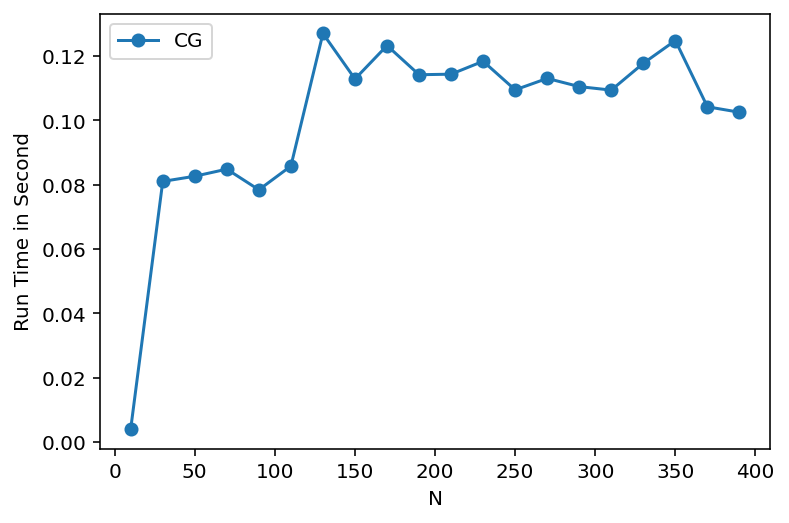
\includegraphics[width=0.5\linewidth]{runtime.png}
	\caption{平均运行时间}
\end{figure}

\subsection{与高斯-赛德尔迭代法的比较}

按前述测试条件,同时使用高斯赛德尔法和共轭梯度法解方程组,并记录运行时间,可以得到
图~\ref{fig:rt_cmp}。
\begin{figure}[htbp]
	\centering
	\label{fig:rt_cmp}
	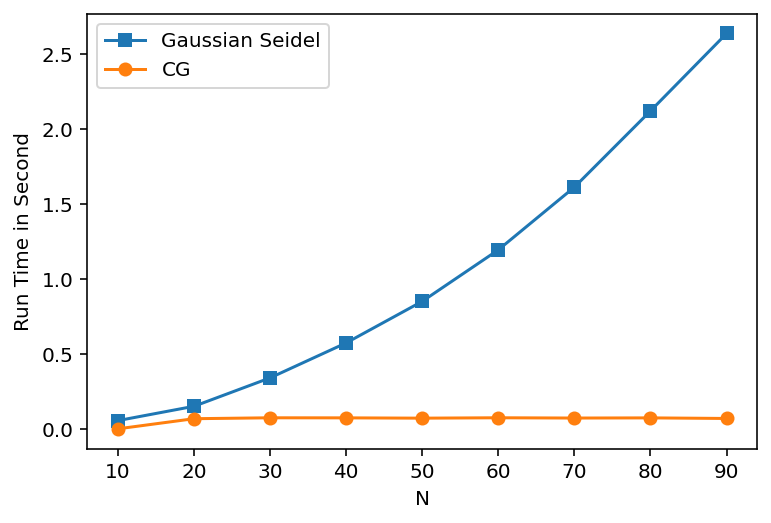
\includegraphics[width=0.5\linewidth]{runtime_cmp.png}
	\caption{平均运行时间比较}
\end{figure}
可以发现,在问题规模较小的情况下,高斯赛德尔法与共轭梯度法运行效率相近。随着
问题规模的扩大,高斯赛德尔法的运行时间会比共轭梯度法的运行时间更长,呈指数级
增长。这表明高斯赛德尔迭代法的迭代次数较为不稳定,并且快速增长,难以解决规模
较大的问题。

\section{结论}

通过实际实现和测试可以发现,在系数矩阵正定时共轭梯度法是一个既方便实现,又高效的
方程组解法。它的迭代次数较少,运行速度较快。

\clearpage

\appendix

\section{附录:代码}
\label{sec:app_code}

\subsection{共轭梯度实现}
\begin{lstlisting}[language=Python,numbers=left,style=PythonStyle,label={code:cg},caption=共轭梯度实现]
import numpy as np


class Equation:
    def __init__(self, coeff, vals):
        self.a = np.asmatrix(coeff, dtype=np.float)
        self.b = np.asarray(vals, dtype=np.float)
        self.solve = self._solve_cg
        assert self.a.shape[1] == self.b.shape[0]

    def use_naive(self):
        self.solve = self._solve_naive
        return self

    def use_conjugate_gradient(self):
        self.solve = self._solve_cg
        return self

    def _solve_naive(self, x0=None, max_iter=512):
        x = x0
        if x0 is None:
            x = np.zeros_like(self.b, dtype=np.float)

        n = self.a.shape[0]
        iter = 0
        prev_x = x.copy()
        while iter < max_iter:
            for j in range(0, n):
                d = self.b[j]

                for i in range(0, n):
                    if j != i:
                        d -= self.a[j, i] * x[i]
                x[j] = d / self.a[j, j]

            if np.allclose(x, prev_x, rtol=1e-5, atol=1e-5, equal_nan=True):
                return x
            prev_x = x.copy()
            iter += 1

        return x

    def _solve_cg(self, x0=None, max_iter=512):
        if x0 is None:
            x0 = np.zeros_like(self.b, dtype=np.float)

        a = np.asmatrix(self.a, dtype=np.float)
        b = np.asmatrix(self.b, dtype=np.float).transpose()
        x = np.asmatrix(x0, dtype=np.float).transpose()

        r = b - a * x
        p = r

        zeros = np.zeros_like(x)

        iter = 0
        while iter <= max_iter:
            if np.allclose(r, zeros):
                break

            ap = a * p

            if np.allclose(ap, zeros):
                break

            alpha = ((r.transpose() * r) / (p.transpose() * ap))[0, 0]

            x += alpha * p

            r1 = r - alpha * ap

            beta = ((r1.transpose() * r1) / (r.transpose() * r))[0, 0]

            p = r1 + beta * p

            r = r1
            iter += 1

        return x


\end{lstlisting}


\end{spacing}

\end{document}